\documentclass[../../tesis_maestria]{subfiles}
\begin{document}
\section{Curvas el\'ipticas}

En esta secci\'on repasamos algunas definiciones y resultados que vamos a requerir acerca
de las curvas el\'itpicas. No demostramos todas las propiedades para mantener esta secci\'on breve,
pero habr\'a referencias para las pruebas omitidas.

\subsection{Definiciones preliminares}\label{sec:preliminares_curvas}%%%%%%%%%%%%%%%%%%%%%%%%%%

\begin{defin}
  Una \emph{curva el\'iptica} $E=(E,O)$ es una curva proyectiva suave de g\'enero 1 con un punto
  distinguido $O\in E$. Decimos que $E$ \emph{est\'a definido sobre} un campo $K$, si $E$ est\'a
  definido sobre $K$ como variedad proyectiva; esto lo denotamos por $E/K$. Una funci\'on no
  constante $\varphi:E\ra E'$ entre curvas el\'ipticas sobre $K$ es una \emph{isogenia} si
  $\varphi$ es un morfismo de variedades sobre $K$ tal que $\varphi(O)=O'$.
\end{defin}

A cada curva el\'iptica se le puede asociar una ecuaci\'on de la forma
\[
  y^2+a_1xy+a_3y=x^3+a_2x^2+a_4x+a_6
\]
donde, si $E$ est\'a definido sobre $K$, $a_i\in K$. De hecho, la homogenizaci\'on de esta
ecuaci\'on es el polinomio que define la imagen de $E$ bajo un encaje
$E\hookrightarrow\PP^2(K)$,\footnote{El espacio proyectivo de dimensi\'on $n$ sobre $K$ se define
  como el espacio cociente $(K^{n+1}-\{0\})/K^*$ donde la acci\'on
  $K^*\curvearrowright(K^{n+1}-\{0\})$ es por multiplicaci\'on escalar $(\la,v)\mapsto\la v$.}
es decir $E$ se puede encajar como una curva c\'ubica suave en $\PP^2(K)$ con ecuaci\'on
\begin{equation}\label{eq:weierstrass-homogenizada}
  y^2z+a_1xyz+a_3yz^2=x^3+a_2x^2z+a_4xz^2+a_6z^3.
\end{equation}
Más precisamente tenemos el siguiente teorema:\marginpar{este teorema es nuevo}

\begin{thm}\label{thm:eq-weierstrass-E}
	Sea $(E,O)$ una curva elíptica sobre $K$ y sea $K(E)$ su campo de funciones de $E$. Entonces existen $x,y\in K(E)$ tales que $x$ (resp. $y$) tiene un polo de orden 2 (resp. 3) en $0$ y tales que $K(E)=K(x,y)$ y tal que la función racional
	\[
		\varphi:E(\ol{K})\ra\PP^2(\ol{K})\quad\mathrm{definido}\;\mathrm{por}\quad \varphi(P)=[x(P),y(P),1] 
	\]
	induce un isomorfismo de $E$ a la curva $\Cc$ sobre $K$, definida por una ecuación de Weierstrass
	\begin{equation}\label{eq:weierstrass-asociada-E}
		y^2+a_1 XY+a_3Y=X^3+a_2X^2+a_4X+a_6,
	\end{equation}
	donde $a_i\in K$ y $\varphi(O)=[0,1,0]$.
	
	Además, cualesquiera dos ecuaciones de Weierstrass que definen una curva elíptica, están relacionadas por el un cambio de variable de la forma:
	\[
		X=u^2X'+r,\quad Y=u^3Y'+su^2X'+t,
	\]
	donde $u\in K^*$ y $r,s,t\in K$.
\end{thm}

\begin{proof}
	Solamente comentamos sobre la primera parte de la prueba, que es una aplicación estándar del teorema de Riemann-Roch, y nos referimos a la fuente original \cite[III.3.1]{SilvermanTAOEC} para la prueba completa del teorema.
	
	Consideramos los divisores de $E$ de la forma $nO$ que tienen grado $n>0$. Como $E$ es de género 1, el teorema de Riemann-Roch nos dice que $\dim\Ll(nO)=n$. De esta manera $\dim\Ll(2O)=2$ y como la función constante $1\in\Ll(2O)$, podemos encontrar un $x\Ll(2O)$ tal que $\{1,x\}$ es una $K-$base de $\Ll(2O)$; observe que $x$ necesariamente tiene un polo de orden 2 en $O$ porque si el polo fuera de orden 1, $\{1,x\}$ no genera a $\Ll(2O)$. Por otro lado podemos extender el conjunto linealmente independiente $\{1,x\}\in\Ll(3O)$ a una base $\{1,x,y\}$; similarmente $y$ tiene un polo de orden 3 en $O$.
	
	Por último, $\{1,x,y,x^2,xy,y^2,x^3\}\subset\Ll(6O)$ es un conjunto de 7 elementos en un espacio de dimensión 6 y por lo tanto existe una combinación lineal no trivial
\begin{equation}\label{eq:comblinealxy}
	A_1+A_2x+A_3y+A_4x^2+A_5xy+A_6y^2+A_7x^3=0,\qquad A_i\in K\;\;\text{no todas}\;=0
\end{equation}
Observe que si $A_6\neq0$ entonces $A_7 x^3$ sería el único término de \eqref{eq:comblinealxy} con un polo de orden 6, el más alto de los órdenes, por lo tanto la suma del lado izquierdo tendría que ser una función meromorfa con un polo de orden 6, no la constante 0. De manera análoga concluimos que $A_7\neq0$.

Después de hacer el cambio de variable
\begin{equation}\label{eq:cambio-variable-weierstrass-general}
	x\mapsto -A_6A_7x,\quad y\mapsto A_6A_7^2y
\end{equation}
a \eqref{eq:comblinealxy} y cancelar el denominador $A_6^3A_7^4$ de la ecuación que surge, obtenemos la ecuación de Weierstrass:
\[
	y^2\underset{a_1}{\underbrace{-\frac{A_5}{A_6A_7}}}xy
	\underset{a_3}{\underbrace{-\frac{A_3}{A_6^2A_7^2}}}y
	=x^3
	\underset{a_2}{\underbrace{-\frac{A_4}{A_6^2A_7^3}}}x^2
	+\underset{a_4}{\underbrace{\frac{A_2}{A_6^2A_7^3}}}x
	\underset{a_6}{\underbrace{-\frac{A_0}{A_6^2A_7^3}}}
\]

El siguiente paso es probar que $\varphi$ es un isomorfismo de curvas sobre su imagen que, por la ecuación anterior, cae dentro de la variedad proyectiva definida por los ceros de \eqref{eq:weierstrass-asociada-E}, pero aquí dejamos la exposición y referimos al lector a \cite{SilvermanTAOEC}.

Solamente comentamos que si a priori tenemos funciones $x,y\in K(E)$ con polos de orden 2 y 3 respectivamente y ningún otro polo ni cero, entonces $\{1,x\}$ y $\{1,x,y\}$ son bases de $\Ll(2O)$ y $\Ll(3O)$ respectivamente y la prueba procede idénticamente. Por lo tanto si de antemano conocemos a $x$ y a $y$ y satisfacen una relación algebraica de la forma \eqref{eq:weierstrass-asociada-E}, entonces esa relación algebraica define una curva elíptica isomorfa a $E$. Este método lo usaremos en la sección \ref{sec:3-5}.
\end{proof}

La ecuación \ref{eq:weierstrass-asociada-E} asociada a $E/K$ se llama la \emph{ecuación de Weierstrass generalizada} de $E$. Si la característica de $K$ es distinto de 2 el cambio de variable
\[
	X'=X,\quad Y'=\frac{1}{2}(Y-a_1X-a_3)
\]
transforma la ecuación de Weierstrass a la forma:
\begin{equation}\label{eq:weierstrass-semi-simple}
  Y'^2=4X'^3+b_2X'^2+b_4X'+b_6,
\end{equation}
donde
\[
	b_2=a_1^2+4a_2,\quad b_4=2a_4+a_1a_3,\quad b_6=a_3^2+4a_6.
\]
Si además la característica de $K$ es distinto de 3 podemos simplificar la ecuación aun más con el cambio de variable
\[
	X=\frac{x-3b_2}{36},\quad Y=\frac{Y'}{108},
\]
que nos da la \emph{ecuación de Weierstrass simplificada} de $E$:
\[
	Y^2=X^3+Ax+B,
\]
donde los coeficientes están definidos por $A=-27c_4$ y $B=-54c_6$ con:
\[
	c_4=b_2^2-24b_4,\qquad c_6-b_2^3+36b_2b_4-216b_6.
\]
\begin{defin}
  Sea $E$ una curva el\'iptica sobre $K$ con una ecuación de Weierstrass simplificada $Y^2=X^3+AX+B$ con $A,B\in K$. El \emph{discriminante} (denotado por $\Delta$) y el $j$-\emph{invariante} (denotado por $j(E)$) de la curva $E$ se definen como:
  \[
    \Delta=-16(4A^3+27B^2) \qquad j(E)=-1728\frac{64 A^3}{\Delta}.
  \]
\end{defin}

El $j$-invariante obtiene su nombre gracias al siguiente teorema importante:

\begin{thm}\label{thm:clasificar-j-invariante}
  Sean $E$ y $E'$ curvas el\'ipticas definidas sobre un campo $K$ algebraicamente cerrado.
  Entonces
  \[
    E\cong E' \quad \iff \quad j(E)=j(E'). 
  \]  
\end{thm}
\noindent (cf. \cite[\S3.1, proposici\'on 1.4]{SilvermanTAOEC} o
\cite[cap\'itulo IV, teorema 4.1]{HartshorneAG} para una prueba usando herramientas de geometr\'ia
algebraica)

Los puntos de $E$ forman un grupo abeliano (cf. \cite[\S3.2]{SilvermanTAOEC}). Para definir la operación geometricamente nos basamos en el celebrado teorema de Bézout\footnote{Este teorema es famoso y se encuentra en muchos textos sobre curvas, por ejemplo en $\S 5.3$ de\cite{FultonAC}} que, en nuestro caso, dice que la cantidad de puntos, contando multiplicidad, en la intersección de $E\subset\PP^2$ con una recta $L\subset\PP^2$ es tres.

Antes de elaborar este argumento, primero consideremos un ecuación de Weierstrass de la forma \ref{eq:weierstrass-semi-simple} escrita sin tanta notación como:
\begin{equation}\label{eq:weierstrass-ss}
	E: Y^2=4X^3+aX^2+bX+c.
\end{equation}
	
Si homogenizamos esta ecuación con la variable $Z$ e intersectamos con la recta al infinito definida por $Z=0$, obtenemos la ecuación $X^3=0$ que tiene una única solución $[0,1,0]\in\PP^2(K)$ de multiplicidad tres. Por el teorema de Bézout, esto quiere decir que la curva $E$ intersecta a la recta al infinito en solamente en $O=[0,1,0]$; el punto $O$ va a ser el nuetro de la operación de grupo de $E$.

Con esto en mente podemos considerar la parte afín de $E$ y agregarle el punto $O$ al infinito. Entonces sean $P$ y $Q$ puntos sobre la curva afín definida por la ecuación \ref{eq:weierstrass-ss}. Sus coordenadas las denotamos por $P=(x(P),y(P))$ y $Q=(x(Q),y(Q))$. Ahora tomamos $L$ la recta en el plano afín que contiene a $P$ y a $Q$; si $P=Q$ tomamos la recta tangente a $P=Q$. Por el teorema de Bezhout hay un tercer punto de intersección que puede ser $O$ ó un tercer punto $R$ en la curva afín.

Si el tercer punto de intersección es $O$, definimos $P+Q=O$ o de otra manera $-P:=Q$. En este caso la recta $L$ es vertical y por lo tanto
\[
	x(-P)=x(P),\qquad y(-P)=-y(P),
\]
que se deduce de la ecuación afín que define a $E$.

Si el tercer punto de intersección es un punto afín $R$, definimos $P+Q=-R$ donde $-R$ es el punto construido arriba, i.e. el tercer punto sobre la recta que une $R$ y $O$. Véase la figura \ref{fig:suma-curva-eliptica} para una ilustración de este proceso sobre la curva elíptica definida por $y^2=x^3+17$.

\begin{figure}\centering
\begin{minipage}[t]{0.3\textwidth}
	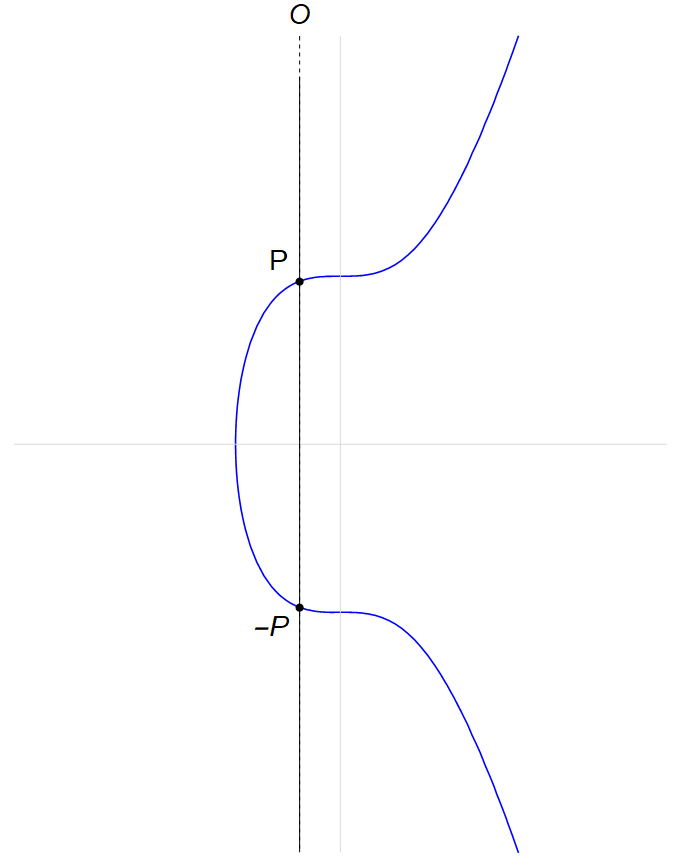
\includegraphics[width=\textwidth]{figuras/suma_eliptica_0}
\end{minipage}
\begin{minipage}[t]{0.3\textwidth}
	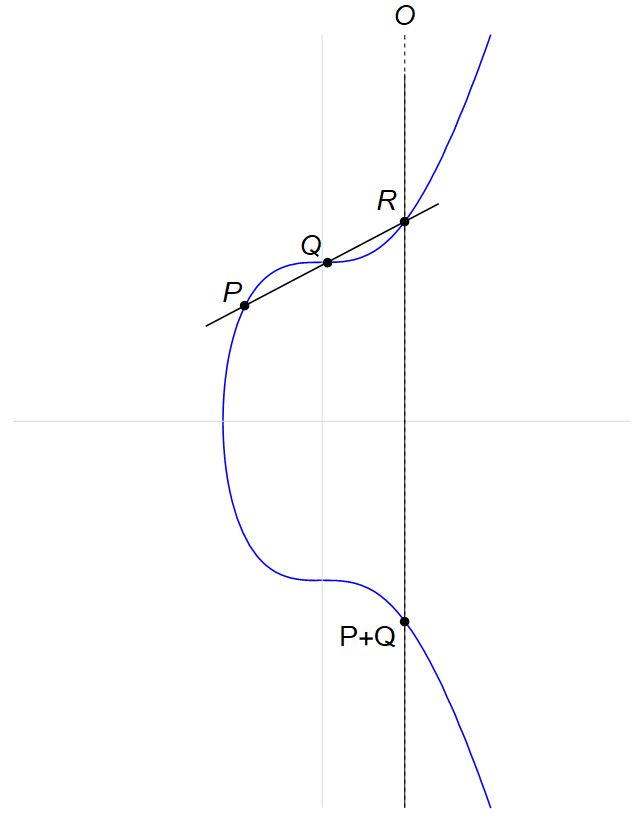
\includegraphics[width=\textwidth]{figuras/suma_eliptica_1}
\end{minipage}
\begin{minipage}[t]{0.3\textwidth}
	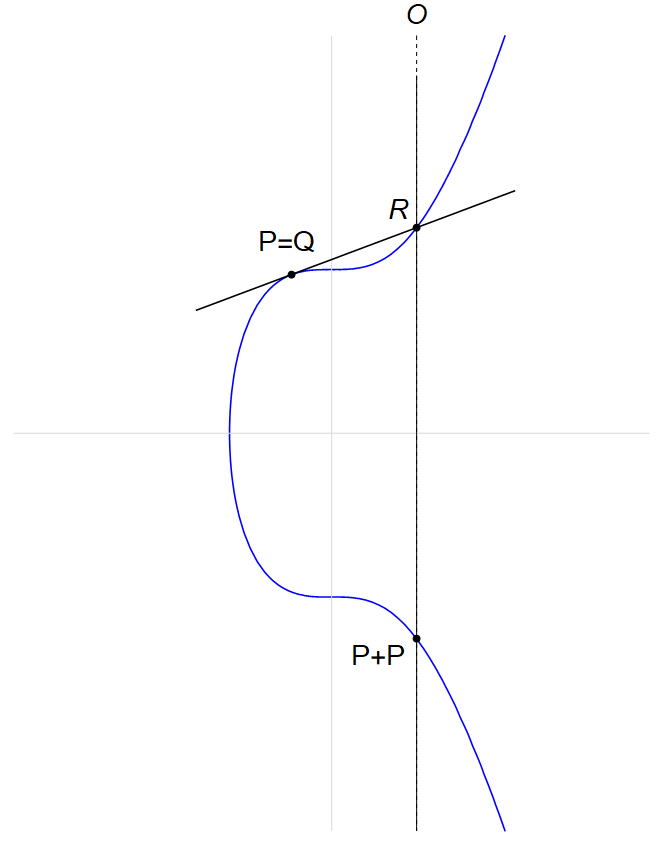
\includegraphics[width=\textwidth]{figuras/suma_eliptica_2}
\end{minipage}
\caption{Construcción geométrica de la suma de puntos $P$ y $Q$ sobre una curva elíptica según si $P+Q=O$, $P\neq Q$ y $P=Q$ respectivamente.}
\label{fig:suma-curva-eliptica}
\end{figure}

Para calcular las coordenadas de $P+Q$ en téminos de las coordenadas de $P$ y $Q$, sea $y=\la x+\mu$ la ecuación de la recta $L$. Como pasa por $P$ y $Q$, su pendiente y su intersección con el eje $y$ son respectivamente:
\[
	\la=\frac{y(Q)-y(P)}{x(Q)-x(P)},\qquad \mu=y(P)-\la x(P)=y(Q)-\la x(Q).
\]
Si sustituimos $y=\la x+\mu$ en la ecuación de Weierstrass \eqref{eq:weierstrass-ss} obtenemos:
\[
	0=x^3+(a-\la^2)x^2+(b-2\la\mu)x+(c-\mu^2).
\]
Por otro lado, como $P,Q$ y $P+Q$ están sobre $L$, las coordenadas $x(P),x(Q)$ y $x(P+Q)$ son raices a la ecuación cúbica anterior. Por lo tanto el polinomio cúbico mónico se factoriza como $(x-x(P))(x-x(Q))(x-x(P+Q))$. Al igualar los coeficientes de ambas expresiones obtenemos el siguiente sistema de ecuaciones:
\begin{gather}
	x(P)+x(Q)+x(P+Q)=\la^2-a, \label{eq:coord-P+Q}\\
	x(P)x(Q)+x(P)x(P+Q)+x(Q)x(P+Q)=b-2\la\mu,\nonumber\\
	x(P)x(Q)x(P+Q)=\mu^2-c, \label{eq:prod-coord-P+Q}
\end{gather}
donde \eqref{eq:coord-P+Q} nos dice que $x(P+Q)=\la^2-a-x(P)-x(Q)$ cuando $P\neq Q$. La fórmula \eqref{eq:prod-coord-P+Q} la usaremos en la sección \ref{sec:3-5}. Cuando $P=Q$, tenemos la fórmula de duplicación:
\begin{equation}
	x(2P)=\frac{x^4-2bx^2-8cx+b^2-4ac}{4x^3+4ax^2+4bx+4c}.
\end{equation}

La construcción geométrica de la suma implica inmediatamente que $O$ es el neutro de la operación. Por otro lado, probar que la operación es asociativa y conmutativa es tedioso porque involucra muchas cálculos que no ilustran la teoría. Nos referimos a la sección III.2 de \cite{SilvermanTAOEC} para las pruebas. 

Las isogenias resultan estar estrechamente relacionadas con la estructura de grupo de las curvas elípticas:

\begin{thm}\label{thm:kernel-isogenias}
	Sea $\varphi: E\ra E'$ una isogenia de curvas elípticas, entonces cumple:
	\begin{enumerate}[label=\roman*)]
		\item Para todos $P,Q\in E$, tenemos $\varphi(P+Q)=\varphi(P)+\varphi(Q)$, es decir $\varphi$ es un homomorfismo de grupos.
		\item El núcleo $\ker\varphi$ es un subgrupo finito de $E$.
		\item Conversamente, para todo subgrupo finito $C$ de $E$ existe una única curva elíptica, denotada por $E/C$, y una isogenia $\varphi bE\ra E/C$ con $\ker\varphi =C$. 
	\end{enumerate}
\end{thm}
\begin{proof}
	La  prueba de las tres partes son III.4.8, III.4.9 y III.4.12 de \cite{SilvermanTAOEC} respectivamente. Solamente mencionamos un comentario adicional que hace Silverman: si $E$ está definido sobre $K$ y $C$ es $\Gal(\ol{K}/K)-$invariante, entonces $E/C$ y $\varphi$ se pueden definir sobre $K$.
\end{proof}

\begin{nota}
	Hay una manera de definir una ecuación de $E/C$, en términos de las coordenadas de los puntos de $C$. En 1971, Jaques Vélu calculó las ecuaciones que definen la curva elíptica $E/C$. Más precisamente, Vélu definió los generadores del campo de funciones de $E/C$ como:
	\[
		X(P):=x(P)+\sum_{Q\in C-\{O\}} x(P+Q)-x(Q),\qquad Y(P):=y(P)+\sum_{Q\in C-\{O\}} y(P+Q)-y(Q).
	\]
Véase \cite{VeluIECE} para más detalles.
\end{nota}

Otra manera de definir la suma de $E$ es con divisores:

\begin{defin}
  Un \emph{divisor} $D$ de $E$ es un elemento del grupo libre abeliano generado por los puntos de
  $E$, es decir $D$ es una suma formal de la forma:
  \[
    D=\sum_{P\in E}n_p(P)
  \]
  donde $n_P\in\ZZ$ y $n_P=0$ para casi toda $P\in E$. Aqu\'i estamos escribiendo $(P)$ como el divisor
  asociado al punto $P$ (i.e. donde $n_Q=0$ para toda $Q\neq P$ y $n_P=1$). Al conjunto de todos los
  divisores de $E$ lo denotamos Div$(E)$.
\end{defin}

Por ejemplo, si $f$ es una funci\'on racional de $E$, es decir un elemento de $K(E)$ distinto de
cero, entonces podemos definir un divisor:
\[
  \mathrm{div}(f):=\sum_{P\in E}\nu_P(f) (P)
\]
donde $\nu_P$ es la valoraci\'on asociada a $K[E]_P$, la localizaci\'on de $K[E]$ (el anillo de
coordenadas de $E$) en el ideal maximal $\m_P=\{f\in K[E]\mid f(P)=0\}$. Recuerda que como $E$
es suave, $K[E]_P$ es un anillo de valoraci\'on discreto.\footnote{Por definici\'on, un punto
  $x$ en una variedad $X$ es no-singular si el anillo local $\Oo_{x,X}$ es un anillo \emph{regular}
  (i.e. el $(\Oo_{x,X}/\m_{x,X})$-espacio vectorial $\m_{x,X}/\m_{x,X}^2$ es de dimensi\'on
  dim$(\Oo_{x,X})$). Como las curvas el\'ipticas son de dimensi\'on 1, ser regular es equivalente
  a ser un anillo de valoraci\'on discreta (cf. \cite[\S9,proposici\'on 9.2]{AtiyahITCA}).}
De esta manera, para un $f\in K[E]_P$ la valoraci\'on $\nu_P(f)$ se define como el \'unico entero
$n$ tal que $f\in\m_P^n$ pero $f\not\in\m_P^{n+1}$.

\begin{defin} Un divisor $D$ de $E$ es \emph{principal} si existe una funci\'on racional
  $f\in K(E)$ distinto de cero tal que $D=$div$(f)$. Adem\'as hay una relaci\'on
  de equivalencia sobre Div$(E)$: decimos que $D$ y $D'$ son \emph{linealmente equivalentes},
  i.e. $D\sim D'$, si $D-D'$ es un divisor principal. El conjunto de clases de equivalencia
  es un grupo abeliano, se llama  el \emph{grupo de Picard} de $E$ y se denota por Pic($E$).
\end{defin}
\noindent Observa que el conjunto de divisores principales es un subgrupo de Div$(E)$ y Pic($E$) es el
grupo cociente con el subgrupo de divisores principales. Enunciamos una caracterizaci\'on de ser
divisor principal:

\begin{prop}\label{prop:divisor_principal}
  Sea $E$ una curva el\'iptica y $D=\sum n_P(P)$ un divisor de $E$. Entonces $D$ es principal
  si y solo si $\sum n_P=0$ y $\sum [n_p]P=O$ (la segunda suma es en $E$).
\end{prop}
\noindent (cf. \cite[cap\'itulo III, \S3, corolario 3.5]{SilvermanTAOEC})

\begin{nota}
La función $D\mapsto \sum n_P$ es importante, entonces le damos un nombre:
\[
	\deg:\text{Div}(E)\ra\ZZ\quad\text{definido por}\quad \deg\paren{\sum_{P\in E}n_P(P)}=\sum_{P\in E}n_P.
\]
Observa que $\deg$ es aditiva, i.e. $\deg(D+D')=\deg(D)+\deg(D')$ para todas $D,D'\in\text{Div}(E)$. 
\end{nota}

Ahora regresamos a la operaci\'on algebraica de $E$. Para $P,Q\in E$ se puede probar que $P+Q$ es
el \'unico punto $R\in E$ tal que $(P)+(Q)\sim (R)+(O)$.

Como $E$ es un grupo abeliano, $E$ es un $\ZZ$-m\'odulo, es decir hay multiplicaci\'on por $N\in\ZZ$.
M\'as precisamente, existen los morfismos de multiplicaci\'on:
\[
  [N]:E\lra E \quad\text{definido por}\quad
  [N]P=\underset{N\,\text{veces}}{\underbrace{P+\cdots+P}}\quad(N>0).
\]
Si $N<0$ definimos $[N]P:=-\big([\abs{N}]P\big)$ y si $N=0$ definimos $[0]P=O$. La m\'ultiplicaci\'on
por $N\in\ZZ$ nos permite estudiar el grupo de torsi\'on de $E$.

\begin{defin}
  Al subgrupo de elementos de $E/K$ de orden $N$ lo denotamos por:
  \[
    E[N]=\ker[N]=\{P\in E(K)\mid [N]P=O\}.
  \]
  El grupo de torsi\'on de $E$ es simplemente la uni\'on de todas las $E[n]$. De la misma
  manera, definimos
  \[
    E[N](\ol{K})=\{P\in E(\ol{K})\mid [N]P=O\}.
  \]
\end{defin}

La estructura de $E[N]$ es relativamente sencilla:

\begin{prop}\label{prop:estructura_EN}
  Sea $E$ una curva el\'iptica sobre $K$ y sea $c=\mathrm{char}(K)$, entonces:
  \[
    E[N]\cong \frac{\ZZ}{N\ZZ}\times\frac{\ZZ}{N\ZZ}
  \]
  si $c=0$ o si $c\nmid N$ cuando $c>0$.
\end{prop}

\begin{proof}
  Nada m\'as probamos el caso cuando $K\subseteq\CC$. Por el teorema de uniformizaci\'on
  (teorema \ref{thm:unif}), existe una latiz tal que $E(\CC)\cong\CC/\Lambda$ pero este cociente
  es isomorfo a $\RR/\ZZ\times\RR/\ZZ$. Por lo tanto $E[N]$ es un subgrupo
  de $E[N](\CC)=\{P\in E(\CC)\mid [N]P=O\}$ que a su vez es un subgrupo (cuyos elementos son de orden
  $N$) de $\RR/\ZZ\times\RR/\ZZ$. El \'unico subgrupo que cumple esto es $\ZZ/N\ZZ\times\ZZ/N\ZZ$.
\end{proof}

En particular, si $\ell$ es un n\'umero primo, entonces $[\ell]:E\ra E$ se restringe a un morfismo
de grupos $[\ell]:E[\ell^{m+1}]\ra E[\ell^m]$ para toda $m>1$. La familia de morfismos
\[
  \begin{tikzcd}
    \cdots \arrow[r] & E\text{[}\ell^{m+2}\text{]} \arrow[r,"\text{[}\ell\text{]}"] &
    E\text{[}\ell^{m+1}\text{]} \arrow[r,"\text{[}\ell\text{]}"] &
    E\text{[}\ell^{m}\text{]} \arrow[r,"\text{[}\ell\text{]}"] &
    \cdots \arrow[r,"\text{[}\ell\text{]}"] & E\text{[}\ell\text{]}
  \end{tikzcd}
\]
es un sistema inverso. Por lo tanto existe su l\'imite inverso:

\begin{defin}
  Sea $E/K$ una curva el\'iptica y $\ell$ un n\'umero primo distinto de la caracter\'istica de $K$.
  El \emph{m\'odulo de Tate} $\ell$-\emph{\'adico} de $E$ se define como:
  \[
    T_{\ell}(E)=\varprojlim_{m}E[\ell^m]
  \]
\end{defin}
Observa que $\ZZ_{\ell}$, los enteros $\ell$-\'adicos, son el l\'imite inverso de los cocientes
$\ZZ/\ell^m\ZZ$, entonces:
\[
  T_{\ell}(E)\cong \ZZ_{\ell}\times\ZZ_{\ell} \quad(\text{char}(K)\neq\ell).
\]
En particular $T_{\ell}(E)$ es un $\ZZ_{\ell}-$m\'odulo libre de rango 2. Si elegimos una
$\ZZ_{\ell}$-base, entonces todos los $v\in T_{\ell}(E)$ se pueden expresar como
$v=(v_1,v_2)\in\ZZ_{\ell}\times\ZZ_{\ell}$. Entonces el determinante
$\det:T_{\ell}(E)\times T_{\ell}(E)\ra\ZZ_{\ell}$, definido por
\[
  \det(v,v'):=\det\begin{pmatrix}v_1&v_1'\\v_2&v_2'\end{pmatrix}=v_1v_2'-v_1'v_2
\]
es una funci\'on bilineal
no-degenerada y alternante sobre el m\'odulo de Tate (y es independiente de la elecci\'on de la
$\ZZ_{\ell}-$base). Hay otra funci\'on
bilineal no-degenerada alternante sobre $T_{\ell}(E)$ que resulta m\'as \'util que el determinante:
el emparejamiento de Weil. Para poder definirlo, necesitamos regresar a $E[m]$, construir ah\'i
el emparejamiento de Weil y despu\'es pasar al l\'imite inverso.

Sean $P,Q\in E[m]$ (donde posiblemente $P=Q$). Elige $g\in\overline{K}(E)$ tal que:
\[
  \mathrm{div}(g)=[m]^*(Q)-[m]^*(O)
\]
donde
\[
  [m]^*:\mathrm{Div}(E)\ra\mathrm{Div}(E) \quad\text{se define en generadores como}\quad
  (R)\mapsto \sum_{S\in[m]^{-1}(R)}e_{[m]}(S)(S)
\]
donde $e_{[m]}(R)$ es el \'indice de ramificaci\'on de $[m]:E\ra E$ en $R\in E$. Con esto definimos
el emparejamiento de Weil como:
\[
  e_m:E[m]\times E[m]\ra \mu_m \quad\text{definido por} \quad e_m(P,Q)=\frac{g(X+P)}{g(X)}
\]
donde $\mu_m\subset\CC$ es el grupo de raices $m$-\'esimas de la unidad y $X\in E$ es un punto
elegido de tal manera que $g$ est\'a bien definido en $X+P$ y en $X$. La funci\'on $e_m$ est\'a
bien definida y no depende de la elecci\'on de $g$ ni de $X$
(cf. \cite[cap\'itulo III, \S8]{SilvermanTAOEC}). La funci\'on $e_m$ cumple las siguientes
propiedades:

\begin{prop}
  El emparejamiento de Weil $e_m$ es una funci\'on bilineal, alternante, no-degenerada, invariante
  bajo la acci\'on del grupo de Galois $\mathrm{Gal}(\overline{K}|K)$ y cumple:
  \begin{equation}\label{eqn:weil_compatible}
    e_{mm'}(P,Q)=e_m\big([m']P,Q\big)
  \end{equation}
\end{prop}
\noindent cf. \cite[cap\'itulo III, proposici\'on 8.1]{SilvermanTAOEC}).

Ahora fijamos un primo $\ell$ (distinto de la caracter\'istica de $K$). Recuerde que los grupos
$\mu_{\ell^n}$, junto con los morfismos $\mu_{\ell^{n+1}}\ra\mu_{\ell^n}$ (definidos por
$\zeta\mapsto\zeta^{\ell}$) forman un sistema inverso: definimos
\[
  T_{\ell}(\mu)=\varprojlim_n \mu_{\ell^n}.
\]
Para ver que podemos tomar l\'imites inversos de ambos lados de
$e_{\ell^n}:E[\ell^n]\times E[\ell^n]\ra\mu_{\ell^n}$, debemos probar que el diagrama
\[
  \begin{tikzcd}[column sep=50]
    E[\ell^{n+1}]\times E[\ell^{n+1}] \arrow[r,"\mathrm{[}\ell\mathrm{]}\times\mathrm{[}\ell\mathrm{]}"]
    \arrow[d,"e_{\ell^{n+1}}"'] &
    E[\ell^n]\times E[\ell^n] \arrow[d,"e_{\ell^n}"] \\
    \mu_{\ell^{n+1}} \arrow[r,"\text{\textasciicircum} \ell"'] & \mu_{\ell^n}
  \end{tikzcd}
\]
es conmutativo: sean $P,Q\in E[\ell^{n+1}]$, entonces
\[
  \big( e_{\ell^{n+1}}(P,Q) \big)^{\ell}=e_{\ell^{n+1}}(P,[\ell]Q)= e_{\ell^n}([\ell]P,[\ell]Q),
\]
donde la primera igualdad es por la linealidad en la segunda variable (escrita multiplicativamente)
y la segunda igualdad es por la f\'ormula (\ref{eqn:weil_compatible}); esto prueba la conmutatividad
del diagrama anterior.

Por lo tanto $e_{\ell^n}$ pasa al l\'imite y obtenemos una funci\'on:
\[
  e_{\ell}:T_{\ell}(E)\times T_{\ell}(E) \ra T_{\ell}(\mu)
\]
que hereda las propiedades de las $e_{\ell^n}$, es decir $e_{\ell}$ es bilineal, no-degenerada,
alternante e invariante bajo la acci\'on del grupo de Galois $G_K$.

La ventaja de usar m\'odulos de Tate y el aparejamiento de Weil, es que podemos calcular los grados
de una isogenia. Sea $\varphi:E\ra E$ una isogenia. Como $\varphi$ es adem\'as un homomorfismo de
grupos, induce un homomorfismo $\varphi_{\ell^n}:E[\ell^n]\ra E[\ell^n]$ y pasando al l\'imite inverso
obtenemos una funci\'on $\ZZ_{\ell}$ lineal $\varphi_{\ell}:T_{\ell}(E)\ra T_{\ell}(E)$. En general
tenemos una funci\'on $\End(E)\ra\End(T_{\ell}(E))$. Con esta notaci\'on tenemos:

\begin{prop}\label{prop:detweil}
  Sea $\varphi\in\End(E)$ y $\varphi_{\ell}\in\End(T_{\ell}(E))$ el morfismo inducido, entonces
  \[
    \det\varphi_{\ell}=\deg\varphi \quad\mathrm{y}\quad
    \tr\varphi_{\ell}=1+\deg\varphi-\deg(1-\varphi)
  \]
\end{prop}

\begin{proof}
  cf. \cite[cap\'itulo III, \S8, proposici\'on 8.6]{SilvermanTAOEC}
\end{proof}



\subsection{Curvas el\'ipticas sobre $\CC$}

En el caso ``geom\'etrico'' ($K=\CC$), las curvas el\'ipticas tambi\'en se pueden describir usando
latices. Un subgrupo aditivo $\Lambda\subset\CC$ es una \emph{ret\'icula} si
$\Lambda\cong\ZZ z_1+\ZZ z_2$ donde $z_1$ y $z_2$ son $\RR$-linealmente independiente o
equivalentement $\im{z_1/z_2}\neq 0$. El cociente $\CC/\Lambda$ es una superficie de Riemann
compacta y como es de esperar, el anillo de funciones meromorfas sobre $\CC/\Lambda$ nos dice
mucho sobre su estructura como variedad. Recuerda que como grupo aditivos:
\[
  \frac{\CC}{\Lambda}\cong\frac{\RR\oplus\RR}{\ZZ\oplus\ZZ}\cong\frac{\RR}{\ZZ}\times\frac{\RR}{\ZZ}
\]


\begin{defin}
  Una funci\'on meromorfa $f:\CC\ra\CC$ es \emph{el\'iptica} (con respecto de $\Lambda$) si es
  $\Lambda$-peri\'odica, es decir
  \[
    f(z+\la)=f(z) \qquad\forall \la\in\Lambda
  \]
  Al conjunto de funciones el\'ipticas lo denotamos $\CC(\Lambda)$. Observa que una funci\'on
  el\'iptica define una funci\'on meromorfa sobre $\CC/\Lambda$
\end{defin}

La funci\'on el\'iptica m\'as importante para clasificar curvas el\'ipticas con latices es la
funci\'on $\wp$ de Weierstrass (asociada a $\Lambda$) definida por:
\[
  \wp_{\Lambda}(z)=\frac{1}{z^2}+
  \sum_{\la\in\Lambda-\{0\}}\paren{\frac{1}{(z-\la)^2}-\frac{1}{\la^2}}.
\]
La funci\'on $\wp$ de Weierstrass es una funci\'on meromorfa cuyos polos (todos de residuo 0)
son exactamente de los puntos de la ret\'icula (cf. \cite[\S1.6, teorema 1.10]{ApostolMFADSINT} o
\cite[cap\'itulo 7, \S 3]{AhlforsCA}).  Por lo tanto induce una funci\'on meromorfa sobre
$\CC/\Lambda$.

La importancia de $\wp$ es que, junto con su derivada, genera a todas las funciones el\'ipticas.
M\'as precisamente, si escibimos $\CC(\wp_{\Lambda},\wp'_{\Lambda})$ como la $\CC$-sub\'algebra de
$\CC(\Lambda)$ generada por $\wp_{\Lambda}$ y su derivada $\wp_{\Lambda}$, entonces tenemos que:
\[
  \CC(\Lambda) = \CC(\wp_{\Lambda},\wp'_{\Lambda}),
\]
(cf. \cite[cap\'itlo VI, teorema 3.2]{SilvermanTAOEC}).

Adem\'as $\wp:=\wp_{\Lambda}$ satisface la ecuaci\'on diferencial
\[
  \wp'^2=4\wp^3-g_2\wp-g_3
\]
donde $g_2=g_2(\Lambda)$ y $g_3=g_3(\Lambda)$ son complejos que dependen de la ret\'icula $\Lambda$.
Esta ecuaci\'on polinomial se parece a la f\'ormula de Weierstrass simplificada; esto no es una
coincidencia:

\begin{thm}\label{thm:unif_part1}
  Sea $\Lambda\subset\CC$ una ret\'icula y sean $g_2=g_2(\Lambda)$ y $g_3=g_3(\Lambda)$ los coeficientes
  de la ecuaci\'on diferencial que cumple $\wp_{\Lambda}$. Entonces la curva $E/\CC$ definida por
  $y^2=4x^3-g_2x-g3$ es el\'iptica (i.e. suave) y $E(\CC)\cong\CC/\Lambda$ como variedades complejas
  bajo la funci\'on
  \[
    z+\Lambda \mapsto [\wp_{\Lambda}(z),\wp'_{\Lambda}(z),1]\in\PP^2(\CC)
  \]
  donde estamos identificando a $E(\QQ)$ con su encaje en $\PP^2(\CC)$. (cf.
  \cite[cap\'itulo VI, proposici\'on 3.6]{SilvermanTAOEC})
\end{thm}

Este teorema le asocia a cada ret\'icula $\Lambda$ una curva el\'iptica $E/\CC$. El resultado inverso
es el teorema de uniformizaci\'on:

\begin{thm}\label{thm:unif}
  Sean $A,B\in\CC$ tales que $4A^3-27B^2\neq0$, entonces existe una ret\'icula $\Lambda\subset\CC$ tal
  que $g_2(\Lambda)=A$ y $g_3(\Lambda)=B$. En particular para cada curva el\'iptica $E:y^2=x^3+Ax+B$
  existe una ret\'icula $\Lambda$ tal que $E(\CC)\cong\CC/\Lambda$ como variedades complejas. Además,
  existe un $\tau\SL_2(\ZZ)\in\HH/\scriptsize{\SL_2(\ZZ)}$ tal que $\Lambda\cong\ZZ\tau\oplus\ZZ$ y
  por lo tanto $E(\CC)\cong\CC/\scriptsize{(\tau\ZZ\oplus\ZZ)}$.
\end{thm}

Los isomorfismos en los teoremas \ref{thm:unif_part1} y \ref{thm:unif} tambi\'en son homomorfismos
de grupo (i.e. de grupos de Lie)





\subsection{Curvas el\'ipticas sobre campos finitos}%%%%%%%%%%%%%%%%%%%%%%%%%%%%%%%%%%%

Para esta secci\'on fijamos un n\'umero primo impar $p$ y fijamos una potencia $q=p^n$ de $p$. De manera
usual, denotamos al campo de Galois de orden $q$ por $\FF_q$. Tambi\'en fijamos una curva el\'iptica
$E$ definida sobre $\FF_q$. Vamos a estar interesados en calcular la cantidad de puntos en $E(\FF_q)$.

Un resultado famoso, debido a Hasse, dice que $\abs{\# E(\FF_q)-q-1}\leq2\sqrt{q}$ (cf.
\cite[cap\'itulo V, teorema 1.1]{SilvermanTAOEC}). En esta secci\'on calcularemos $\# E(\FF_q)$
usando la traza del mapeo de Frobenius que est\'a definido para cualquier curva el\'iptica sobre
un campo finito.

El mapeo de Frobenius usual $\varphi:\FF_q\ra\FF_q$, definido por $x\mapsto x^q$, induce un
automorfismo de $E$ (que denotamos igual) definido en coordenadas afines por
$P=(x,y)\mapsto (x^q,y^q)$. Con esto tenemos:

\begin{thm}\label{thm:traza_frobenius}
  Sea $E/\FF_q$ una curva el\'iptica, $\varphi:E\ra E$ el mapeo de Frobenius de orden $q$ y
  escribe $a_q(E):=q+1-\# E(\FF_q)$. Entonces el morfismo inducido
  $\varphi_{\ell}:T_{\ell}(E)\ra T_{\ell}(E)$ en los m\'odulos de Tate ($\ell\neq p$) tiene polinomio
  caracter\'istico $T^2-a_q(E)T+q$. En particular el mapeo de Frobenius satisface
  $\varphi^2-a_q(E)\varphi+q=0\in\End(E)$.
\end{thm}
\begin{proof}
  Como el grupo absoluto de Galois $G_{\FF_q}$ es generado topol\'ogicamente por el mapeo de
  Frobenius de orden $q$ sobre $\overline{\FF}_q$, entonces $P\in E(\FF_q)$ si y solamente si
  $\varphi(P)=\varphi(x,y)=(x^q,y^q)=(x,y)=P$ o equivalentemente $E(\FF_q)=\ker(1-\varphi)$.

  Ahora como $p\nmid1$, la isogenia $1-\varphi$ es separable (cf.
  \cite[cap\'itulo III, corolario 5.5]{SilvermanTAOEC}) y las isogenias separables cumplen
  que $\#\ker\varphi=\deg\varphi$ (cf. \cite[cap\'itulo III, teorema 4.10.c]{SilvermanTAOEC}),
  tenemos que
  \begin{equation}\label{eq:deg_1menosphi}
    \# E(\FF_q)=\#\ker(1-\varphi)=\deg(1-\varphi).
  \end{equation}
  \begin{nota}
    Como $\deg\varphi=q$ y $\deg:\End(E)\ra\ZZ$ es una forma cuadr\'atica positiva definida, la
    desigualdad de Hasse mencionada anteriormente se sigue de la f\'ormula anterior despu\'es de
    aplicar una versi\'on adecuada de la desigualdad de Cauchy-Schwarz para $\deg$.
  \end{nota}

  Luego aplicamos la proposici\'on \ref{prop:detweil} a \ref{eq:deg_1menosphi} y tenemos que
  $\det\varphi_{\ell}=\deg\varphi=q$ y
  \[
    \tr\varphi_{\ell}=1+\deg\varphi-\deg(1-\varphi)=1+q-\# E(\FF_q)=a_q(E).
  \]
  Por lo tanto el polinomio caracter\'istico de $\varphi_{\ell}$ es $T^2-a_q(E)T+q$.

  Por el teorema de Cayley-Hamilton, $\varphi_{\ell}^2-a_q(E)\varphi_{\ell}+q=0$. Volvemos a aplicar
  la proposici\'on \ref{prop:detweil} para concluir que:
  \[
    \deg(\varphi^2-a_q(E)\varphi+q)=\det(\varphi_{\ell}^2-a_q(E)\varphi_{\ell}+q)=0.
  \]
  La \'unica isogenia de grado cero es $[0]\in\End(E)$ y acabamos.
\end{proof}

Curvas el\'ipticas sobre campos finitas tambi\'en surgen de curvas el\'ipticas definidas sobre $\QQ$
o en general sobre campos locales (i.e. localmente compactos con respecto de una topolog\'ia no
discreta, por ejemplo cualquier extensi\'on finita de $\QQ_p$ para alg\'un primo $p$).

Sea $E/\QQ$ una curva el\'iptica con una ecuaci\'on $y^2=ax^3+bx^2+cx+d$ y sea $p$ primo. Entonces
bajo el cambio de coordenadas $x=ux'+v$, $y=wy'$ (para algunas $u,v,w\in\QQ$) la nueva curva
el\'iptica $E'$ definida por
\[
  (y')^2=aw^{-2}(ux'+v)^3+bw^{-2}(ux'+v)^2+cw^{-2}(ux'+v)+dw^{-2}=a'(x')^3+b'(x')^2+c'x'+d'
\]
es isomorfa a $E$ y los n\'umeros $u,v,w\in\QQ$ se pueden tomar de tal manera que los denominadores
de los nuevos coeficientes sean primos relativos con $p$, ie $a',b',c',d'\in\ZZ_{(p)}$ (la
localizaci\'on de $\ZZ$ en el ideal primo $p\ZZ$). %Por lo tanto podemos asumir sin p\'erdidad de
% generalidad que los coeficientes de la ecuaci\'on de $E$ son a priori elementos de $\ZZ_{(p)}$.

El anillo $\ZZ_{(p)}$ tiene un morfismo de reducci\'on m\'odulo $p$:
\[
  \begin{tikzcd}[column sep=large]
    \ZZ_{(p)} \arrow[r,two heads,"\mathrm{mod}\,p"] &
    \frac{\ZZ_{(p)}}{p\ZZ_{(p)}}\cong\frac{\ZZ}{p\ZZ}=\FF_p.
  \end{tikzcd}
\]
Por lo tanto si tomamos el polinomio $y^2-ax^3-bx^2-cx-d\in\ZZ_{(p)}[x,y]$ que define $E$
(despu\'es de un cambio de coordenadas adecuado) podemos aplicar la reducci\'on m\'odulo $p$ a cada
coeficiente, i.e. aplicar el morfismo $\ZZ_{(p)}[x,y]\epi\FF_p[x,y]$ para obtener un polinomio con
coeficientes en $\FF_p$. En ciertos casos, este procedimiento produce una curva el\'iptica $E_p$
definida sobre un campo finito. Veamos bajo qu\'e condiciones sucede esto.

\begin{defin}
  Sea $E/\QQ$ una cuva el\'iptica y $p$ un primo impar.
  \begin{enumerate}
  \item $E$ tiene \emph{buena reducci\'on} m\'odulo $p$ si existe un cambio de variable tal que
    la nueva ecuaci\'on que define a $E$ cumple $y^2-ax^3-bx^2-cx-d\in\ZZ_{(p)}[x,y]$ y adem\'as
    $a\in\ZZ_{(p)}^*$, de tal manera que la curva el\'iptica $E_p/\FF_p$ es suave (o equivalentemente
    que la ecuaci\'on $y^2=ax^3+bx^2+cx+d\Mod{p}$ tiene tres raices diferentes).
  \item $E$ tiene \emph{reducci\'on multiplicativa} m\'odulo $p$ si existe un cambio de variable
    tal que la nueva ecuaci\'on que define a $E$ cumple $y^2-ax^3-bx^2-cx-d\in\ZZ_{(p)}[x,y]$ y
    adem\'as $a\in\ZZ_{(p)}^*$, de tal manera que la ecuaci\'on $y^2=ax^3+bx^2+cx+d\Mod{p}$ tiene
    una raiz de multiplicidad dos y otra raiz simple.
  \item $E$ tiene \emph{reducci\'on aditiva} m\'odulo $p$ si existe un cambio de variable
    tal que la nueva ecuaci\'on que define a $E$ cumple $y^2-ax^3-bx^2-cx-d\in\ZZ_{(p)}[x,y]$ y
    adem\'as $a\in\ZZ_{(p)}^*$, de tal manera que la ecuaci\'on $y^2=ax^3+bx^2+cx+d\Mod{p}$ tiene
    una raiz de multiplicidad tres.
  \end{enumerate}
  Decimos que $E$ tiene \emph{reducci\'on mala} si satisface 2 o 3. Si $E$ tiene reducci\'on
  multiplicativa, decimos que la reducci\'on es \emph{partida} si las direcciones de las tangentes
  en el nodo son elementos de $\FF_p$ y decimos que es \emph{no-partida} en otro caso.
\end{defin}

\begin{defin}
  Una curva el\'iptica $E/\QQ$ es semiestable en un primo $p$ si tiene reducci\'on buena en $p$
  o reducci\'on multiplicativa partida en $p$. Decimos que $E$ es \emph{semiestable} si es
  semiestable en todo primo.
\end{defin}





\end{document}
